% You must use only one of the following `\documentclass' commands
% For deliverables D2 and D3 you must use the following command:
%
\documentclass[runningheads,a4paper,oribibl]{llncs}
%
%For all other deliverables 
% you must use the command below (and put the one above in comments).
% 
%
%\documentclass[runningheads,a4paper]{llncs}

\usepackage[T1]{fontenc}  %% needed for special characters (umlaut)
\usepackage[latin1]{inputenc}
\usepackage{graphicx}     %% for graphical things such as including pictures
\usepackage{url}          %% for proper formatting of URLs
\usepackage{tikz}
\usetikzlibrary{positioning}

\newcommand{\todo}[1]{\textbf{[TODO: #1]}}
\newcommand{\model}{\texttt{twitter-}\allowbreak\texttt{roberta-}\allowbreak\texttt{base-}\allowbreak\texttt{hate}}
\newcommand{\modelfull}{\texttt{cardiffnlp/}\allowbreak\model}
% Confusion matrix counts
\newcommand{\aaeTN}{1123}
\newcommand{\aaeFP}{3384}
\newcommand{\aaeFN}{75}
\newcommand{\aaeTP}{107}
\newcommand{\mainTN}{8083}
\newcommand{\mainFP}{4136}
\newcommand{\mainFN}{844}
\newcommand{\mainTP}{148}

\begin{document}

\pagestyle{headings}

\mainmatter

\title{Dialect Bias in Hate Speech Detection Systems Audit to Pretained Twitter Classifier on AAE Aligned Text}

\titlerunning{Dialectal Bias in Hate Speech Detection}

\author{S\'{e}rgio Apolin\'{a}rio da Costa}

\institute{
    Department of Computing Science \\
    Ume\aa{} University, Sweden \\
    \email{mai25sca@cs.umu.se}
}

\maketitle

\begin{abstract}
TODO TODO TODO TODO TODO TODO TODO TODO TODO TODO TODO TODO TODO TODO TODO TODO TODO TODO TODO TODO TODO TODO TODO TODO TODO TODO TODO TODO TODO TODO TODO TODO TODO TODO TODO TODO TODO TODO TODO TODO TODO TODO TODO TODO TODO TODO TODO TODO TODO TODO TODO TODO TODO TODO TODO TODO TODO TODO TODO TODO TODO TODO TODO TODO TODO TODO TODO TODO TODO TODO TODO
\end{abstract}

\section{Introduction}
Social media platforms rely on automatic classifiers to detect or remove hateful
content. This systems are usually trained and tested on text that is close to
mainstream written English. Friedman and Nissenbaum define a system biased
when it works well for the population it was built and tested on, but it fails for users
who do not belong to this population. African-American English (AAE)
is a variety of English with its own grammar and vocabulary. If a classifier 
learned its notion of ``toxic'' based on other varieties, it has no reliable way of 
knowing that the AAE expression it has rarely seen is not offensive.

Earlier work has found that hate speech datasets and the models trained on
them treat tweets associated with AAE differently~\cite{davidson2019}.

This project will study the \modelfull{}\footnote{\url{https://huggingface.co/cardiffnlp/twitter-roberta-base-hate}} model, and 
evaluate it on the tweets of Davidson et al.~\cite{davidson2017} dataset.

\subsection{Research Questions}
This project will address the following research questions.
\begin{itemize}
      \item Does the classifier show a performance gap between AAE-aligned and
            tweets? Is the gap larger than sampling noise?
      \item Which factors are linked to the AAE-aligned misclassification?
\end{itemize}

The hypothesis is that the classifier flags more of the AAE-aligned tweets that are
not hate speech compared to the mainstream tweets.

\section{Literature Review}\label{sec:lit}
TODO TODO TODO TODO TODO TODO TODO TODO TODO TODO TODO TODO TODO TODO TODO TODO TODO TODO TODO TODO TODO TODO TODO TODO TODO TODO TODO TODO TODO TODO TODO TODO TODO TODO TODO TODO TODO TODO TODO TODO TODO TODO TODO TODO TODO TODO TODO TODO TODO TODO TODO TODO TODO TODO TODO TODO TODO TODO TODO TODO TODO TODO TODO TODO TODO TODO TODO TODO TODO TODO

\section{Materials and Methods}\label{sec:methods}

\subsection{Overview}
The pipeline has three components with different roles, shown in Figure~\ref{fig:pipeline}.
The Davidson corpus provides the ground truth (human labels). The dialect predictor assigns
each tweet to a group. The RoBERTa hate classifier labels each tweet  as hate or not hate.
The two models run independently on the tweet text and their outputs are joined at the evaluation step.

\begin{figure}
   \centering
   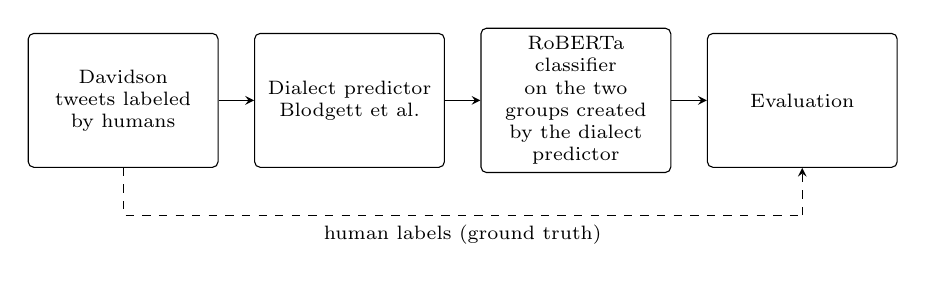
\begin{tikzpicture}[node distance=0.45cm, >=stealth,
       box/.style={draw, rounded corners=2pt, align=center, minimum height=1.7cm, text width=2.2cm, inner sep=3pt, font=\scriptsize}]
     \node[box] (data) {Davidson tweets labeled by humans};
     \node[box, right=of data] (dialect) {Dialect predictor\\ Blodgett et al.\\};
     \node[box, right=of dialect] (clf) {RoBERTa classifier\\ on the two groups created by the dialect predictor};
     \node[box, right=of clf] (eval) {Evaluation};
     \draw[->] (data) -- (dialect);
     \draw[->] (dialect) -- (clf);
     \draw[->] (clf) -- (eval);
     \coordinate (left) at ([yshift=-0.6cm]data.south);
     \coordinate (right) at ([yshift=-0.6cm]eval.south);
     \draw[dashed] (data.south) -- (left) -- node[below, font=\scriptsize] {human labels (ground truth)} (right);
     \draw[->, dashed] (right) -- (eval.south);
   \end{tikzpicture}
   \caption{The pipeline.\label{fig:pipeline}}
\end{figure}

\subsection{Davidson et al. dataset}
In this project it was used the corpus of Davidson et al.~\cite{davidson2017}. This dataset has
24,783 tweets with the full text, each labelled by crowd workers as \textbf{hate speech} (1,430 tweets),
\textbf{offensive language} (19,190) or \textbf{neither} (4,163). Since the classification is binary, 
it will only be mapped the  \emph{hate speech} class to the positive class (hate) and treat both \emph{offensive language} 
and \emph{neither} as not hate. This choice defines what counts as an error throughout the report,
and in the Section~\ref{sec:discussion} this will be further explained.

\subsection{Blodgett et al.}\label{sec:dialect}
To predict the dialect from the tweet, it was used the released model of Blodgett et al.~\cite{blodgett2016}.
This model it was ported from Python 2 to Python 3 without changing the inference logic. 
The model has a vocabulary of 191,874 words and a count table that gives the usage of each
word in the four language groups. The groups are \emph{African-American}, \emph{Hispanic}, \emph{Asian}
and \emph{White}. 

For a tweet, it tokenises the text with a Twitter-specific tokenizer, lowercases it, and keeps
the in-vocabulary tokens. It then infers a probability distribution after seing the full tweet text.
The result is a vector with four probability distributions, and we use the first one, the African-American distribution,
as the \emph{AAE score} of the tweet. Tweets with no in-vocabulary token, or with fewer than 20\% in-vocabulary
tokens, get no score. The score is a bag-of-words, t says how much of the wording resembles African-American-aligned
usage, and it is not the probability that the author is African American.

We define two groups with thresholds on the AAE score. Tweets with a score of at least 0.6 are \emph{AAE-aligned},
tweets with a score of at most 0.4 are \emph{mainstream}, and the tweets in between are \emph{ambiguous}
and excluded. We also exclude 7 tweets that received no score. This leaves 17,900 tweets, of which
4,689 are AAE-aligned and 13,211 are mainstream. 
% We check the sensitivity to these thresholds 
% with stricter values (Section~\ref{sec:sensitivity}).

\subsection{Hate classifier (RoBERTa)}
The audited classifier is \modelfull{}. According to its model card, it is a RoBERTa-base model
pretrained on about 58 million tweets and fine-tuned for binary hate speech detection on the TweetEval
benchmark, that is, on HatEval. We run it as is, with no further
training, through the Hugging Face \texttt{transformers} library.

Before inference, user mentions are replaced by \texttt{@user} and links by \texttt{http}, as in the
preprocessing of the model, and inputs are truncated to 128 tokens. The predicted label is the one the
model returns, which corresponds to the default decision threshold. The model was trained on HatEval,
a corpus collected independently of the Davidson tweets. 
% We did not check for tweet-level overlap between the two.

\subsection{Evaluation}
All metrics treat hate as the positive class, and are computed separately for each group from
the counts of true and false positives and negatives (TP, FP, FN, TN). Table~\ref{tab:metrics-def} defines them.
In this project the difference between the AAE-aligned and the mainstream value of a metric its called \emph{gap}.


To test whether a gap was larger than sampling noise, it was used a non-parametric bootstrap. 
In each of 2,000 rounds, it was drawn each group again with replacement, with the same size 
as the original, it was then computed the metric on both resampled groups and record the gap.
The 95\% confidence interval was given by the 2.5th and 97.5th percentiles of the 2,000 gaps.
The approximate two-sided $p$-value is twice the smaller of the shares of resampled gaps that
are at least zero and below zero. The bootstrap measures only sampling noise, it does not account
for errors of the dialect predictor or of the human labels. It was tested the gaps in F1 and in FPR.

% TODO TODO TODO TODO TODO
% After that was added three more descriptive analyses. First, it was computed the rate of tweets
% flagged as hate within each human label (hate speech, offensive language, neither) and group,
% which compares tweets of the same kind. Second, it was recomputed the FPR gap with stricter dialect
% thresholds. Finally, it was inspected flagged tweets by hand and look at word-level AAE scores.

\begin{table}
   \centering
   \begin{tabular}{|l|l|p{5.2cm}|}
     \hline
     \textbf{Metric} & \textbf{Formula} & \textbf{Meaning}\\
     \hline
     Precision & TP / (TP + FP) & Of the tweets flagged as hate, how many are hate?\\
     Recall & TP / (TP + FN) & Of the hate tweets, how many were caught?\\
     F1 & 2TP / (2TP + FP + FN) & Balance between precision and recall.\\
     Accuracy & (TP + TN) / all & How many tweets are classified correctly?\\
     FPR & FP / (FP + TN) & Of the tweets that are not hate, how many are flagged?\\
     \hline
   \end{tabular}
   \caption{Evaluation metrics. \label{tab:metrics-def}}
\end{table}

\subsection{Implementation}
TODO TODO TODO TODO TODO TODO TODO TODO TODO TODO TODO TODO TODO TODO TODO TODO TODO TODO TODO TODO TODO TODO TODO TODO TODO TODO TODO TODO TODO TODO TODO TODO TODO TODO TODO TODO TODO TODO TODO TODO TODO TODO TODO TODO TODO TODO TODO TODO TODO TODO TODO TODO TODO TODO TODO TODO TODO TODO TODO TODO TODO TODO TODO TODO TODO TODO TODO TODO TODO TODO

\section{Results}\label{sec:results}
\subsection{Groups and label composition}
The Table~\ref{tab:groups} shows how the human labels are distributed over the groups. The two groups
have a very different composition. In the AAE-aligned group, 94.1\% of the tweets are labelled
offensive language, 3.9\% hate speech and 2.0\% neither. In the mainstream group, the corresponding compositions,
are 64.3\%, 7.5\% and 28.2\%. As a consequence, 97.9\% of the AAE-aligned tweets that are not hate are offensive language,
against 69.5\% in the mainstream group.

\begin{table}
   \centering
   \small
   \begin{tabular}{|l|r|r|r|r|}
     \hline
     & \textbf{Hate} & \textbf{Offensive} & \textbf{Neither} & \textbf{Total}\\
     \hline
     All tweets & 1,430 & 19,190 & 4,163 & 24,783\\
     AAE-aligned ($\geq 0.6$) & 182 & 4,412 & 95 & 4,689\\
     Mainstream ($\leq 0.4$) & 992 & 8,495 & 3,724 & 13,211\\
     Excluded & 256 & 6,283 & 344 & 6,883\\
     \hline
   \end{tabular}
   \caption{Davidson et al. dataset by dialect group (thresholds apply to the AAE score).\label{tab:groups}}
\end{table}

\subsection{Metrics per group}
The Table~\ref{tab:confusion} shows the confusion matrices and the Table~\ref{tab:metrics} gives the
metrics at the default threshold of the classifier. The classifier performs poorly on both groups,
with a precision of about 0.03 and an F1 of about 0.06. F1 is practically identical in the two groups.
The other metrics are not. The recall is 0.588 for AAE-aligned tweets and 0.149 for mainstream tweets,
and the FPR is 0.751 against 0.338. Accuracy is 0.262 against 0.623. The classifier is therefore much more
willing to flag AAE-aligned tweets, both the ones that are hate and the ones that are not.

\begin{table}
   \centering
   \begin{tabular}{|l|l|r|r|}
     \hline
     \textbf{Group} & \textbf{Davidson label} & \textbf{Not flagged} & \textbf{Flagged}\\
     \hline
     AAE-aligned & not hate & TN = \aaeTN & FP = \aaeFP\\
      & hate & FN = \aaeFN & TP = \aaeTP\\
     \hline
     Mainstream & not hate & TN = \mainTN & FP = \mainFP\\
      & hate & FN = \mainFN & TP = \mainTP\\
     \hline
   \end{tabular}
   \caption{Confusion matrices at the default threshold.\label{tab:confusion}}
\end{table}

\begin{table}
   \centering
   \begin{tabular}{|l|r|r|r|}
     \hline
     \textbf{Metric} & \textbf{AAE-aligned} & \textbf{Mainstream} & \textbf{Gap}\\
     \hline
     Precision & 0.031 & 0.035 & $-0.004$\\
     Recall & 0.588 & 0.149 & $+0.439$\\
     F1 & 0.058 & 0.056 & $+0.002$\\
     Accuracy & 0.262 & 0.623 & $-0.361$\\
     False positive rate & 0.751 & 0.338 & $+0.412$\\
     \hline
   \end{tabular}
   \caption{Metrics at the default threshold. Gap = AAE-aligned minus mainstream. \label{tab:metrics}}
\end{table}


\subsection{Significance of the gaps}
Table~\ref{tab:bootstrap} shows the bootstrap results. The interval of the F1 gap contains zero and the gap is about as large as the noise (gap-to-noise ratio about 0.1), so there is no evidence of a difference in F1. The interval of the FPR gap is far from zero, and the gap is about 27 times the noise: the sign of the FPR gap did not change in any of the 2,000 resamples. The FPR of AAE-aligned tweets is 2.2 times that of mainstream tweets.

\begin{table}
   \centering
   \begin{tabular}{|l|r|c|r|}
     \hline
     \textbf{Gap in} & \textbf{Observed} & \textbf{95\% bootstrap CI} & \textbf{$p$}\\
     \hline
     F1 & $+0.002$ & $[-0.012, +0.015]$ & 0.73\\
     FPR & $+0.412$ & $[+0.397, +0.428]$ & $<0.001$\\
     \hline
   \end{tabular}
   \caption{Bootstrap test of the gaps (2,000 resamples, seed 42).\label{tab:bootstrap}}
\end{table}

\subsection{Reference points}
Metrics are easier to judge against simple references (Table~\ref{tab:reference}). The classifier
flags 74.5\% of all AAE-aligned tweets and 32.4\% of all mainstream tweets, while the shares of
hate speech according to the labels are 3.9\% and 7.5\%. The precision divided by the share of
hate (the \emph{lift}) is 0.79 and 0.46. A classifier that flags tweets at random would have a lift of 1,
so at the default threshold the flagged tweets contain a smaller share of hate speech than the whole group
does. A model that flags nothing would have an accuracy of 96.1\% and 92.5\%, against the 26.2\%
and 62.3\% observed.

\begin{table}
   \centering
   \begin{tabular}{|l|r|r|}
     \hline
     & \textbf{AAE-aligned} & \textbf{Mainstream}\\
     \hline
     Share of hate speech (labels) & 3.9\% & 7.5\%\\
     Share of tweets flagged by the model & 74.5\% & 32.4\%\\
     Precision lift (precision / share of hate) & 0.79 & 0.46\\
     Accuracy of a model that never flags & 96.1\% & 92.5\%\\
     Hate tweets missed (1 $-$ recall) & 41.2\% & 85.1\%\\
     \hline
   \end{tabular}
   \caption{Reference points for the metrics.\label{tab:reference}}
\end{table}

% \subsection{Within each human label}\label{sec:within}
% TODO TODO TODO TODO TODO TODO TODO TODO TODO TODO TODO TODO TODO TODO TODO TODO TODO TODO TODO TODO TODO TODO TODO TODO TODO TODO TODO TODO TODO TODO TODO TODO TODO TODO TODO TODO TODO TODO TODO TODO TODO TODO TODO TODO TODO TODO TODO TODO TODO TODO TODO TODO TODO TODO TODO TODO TODO TODO TODO TODO TODO TODO TODO TODO TODO TODO TODO TODO TODO TODO

\subsection{Sensitivity to the dialect threshold}\label{sec:sensitivity}
TODO TODO TODO TODO TODO TODO TODO TODO TODO TODO TODO TODO TODO TODO TODO TODO TODO TODO TODO TODO TODO TODO TODO TODO TODO TODO TODO TODO TODO TODO TODO TODO TODO TODO TODO TODO TODO TODO TODO TODO TODO TODO TODO TODO TODO TODO TODO TODO TODO TODO TODO TODO TODO TODO TODO TODO TODO TODO TODO TODO TODO TODO TODO TODO TODO TODO TODO TODO TODO TODO

\subsection{Which words?}\label{sec:words}
TODO TODO TODO TODO TODO TODO TODO TODO TODO TODO TODO TODO TODO TODO TODO TODO TODO TODO TODO TODO TODO TODO TODO TODO TODO TODO TODO TODO TODO TODO TODO TODO TODO TODO TODO TODO TODO TODO TODO TODO TODO TODO TODO TODO TODO TODO TODO TODO TODO TODO TODO TODO TODO TODO TODO TODO TODO TODO TODO TODO TODO TODO TODO TODO TODO TODO TODO TODO TODO TODO

\section{Discussion and Conclusion}\label{sec:discussion}
\subsection{What the results show?}
TODO TODO TODO TODO TODO TODO TODO TODO TODO TODO TODO TODO TODO TODO TODO TODO TODO TODO TODO TODO TODO TODO TODO TODO TODO TODO TODO TODO TODO TODO TODO TODO TODO TODO TODO TODO TODO TODO TODO TODO TODO TODO TODO TODO TODO TODO TODO TODO TODO TODO TODO TODO TODO TODO TODO TODO TODO TODO TODO TODO TODO TODO TODO TODO TODO TODO TODO TODO TODO TODO

\subsection{What explains the gap?}
TODO TODO TODO TODO TODO TODO TODO TODO TODO TODO TODO TODO TODO TODO TODO TODO TODO TODO TODO TODO TODO TODO TODO TODO TODO TODO TODO TODO TODO TODO TODO TODO TODO TODO TODO TODO TODO TODO TODO TODO TODO TODO TODO TODO TODO TODO TODO TODO TODO TODO TODO TODO TODO TODO TODO TODO TODO TODO TODO TODO TODO TODO TODO TODO TODO TODO TODO TODO TODO TODO

\subsection{Limitations}
TODO TODO TODO TODO TODO TODO TODO TODO TODO TODO TODO TODO TODO TODO TODO TODO TODO TODO TODO TODO TODO TODO TODO TODO TODO TODO TODO TODO TODO TODO TODO TODO TODO TODO TODO TODO TODO TODO TODO TODO TODO TODO TODO TODO TODO TODO TODO TODO TODO TODO TODO TODO TODO TODO TODO TODO TODO TODO TODO TODO TODO TODO TODO TODO TODO TODO TODO TODO TODO TODO

\subsection{Future work}\label{sec:future}
TODO TODO TODO TODO TODO TODO TODO TODO TODO TODO TODO TODO TODO TODO TODO TODO TODO TODO TODO TODO TODO TODO TODO TODO TODO TODO TODO TODO TODO TODO TODO TODO TODO TODO TODO TODO TODO TODO TODO TODO TODO TODO TODO TODO TODO TODO TODO TODO TODO TODO TODO TODO TODO TODO TODO TODO TODO TODO TODO TODO TODO TODO TODO TODO TODO TODO TODO TODO TODO TODO

\subsection{Conclusion}
TODO TODO TODO TODO TODO TODO TODO TODO TODO TODO TODO TODO TODO TODO TODO TODO TODO TODO TODO TODO TODO TODO TODO TODO TODO TODO TODO TODO TODO TODO TODO TODO TODO TODO TODO TODO TODO TODO TODO TODO TODO TODO TODO TODO TODO TODO TODO TODO TODO TODO TODO TODO TODO TODO TODO TODO TODO TODO TODO TODO TODO TODO TODO TODO TODO TODO TODO TODO TODO TODO

\bibliographystyle{plain}
\bibliography{references}

\end{document}
